\documentclass[conference]{IEEEtran}

% ================= 日本語対応(LuaLaTeX推奨) =================
\usepackage{luatexja}
\usepackage{luatexja-fontspec}
\IfFontExistsTF{HaranoAjiMincho}{
  \setmainjfont{HaranoAjiMincho}
  \setsansjfont{HaranoAjiGothic}
}{
  \setmainjfont{Noto Serif CJK JP}
  \setsansjfont{Noto Sans CJK JP}
}
\ltjsetparameter{yjabaselineshift=0pt}
\ltjsetparameter{alxspmode={`/,-1}}

% ================= 基本パッケージ =================
\usepackage{graphicx,amsmath,siunitx,booktabs,balance,url,cite}
\usepackage[hidelinks]{hyperref}
\sisetup{detect-all}
\usepackage{physics}
\usepackage{enumitem}

% ================= 図(TikZ / pgfplots) =================
\usepackage{tikz,pgfplots}
\usetikzlibrary{arrows.meta,positioning,calc,patterns}
\pgfplotsset{compat=1.18}

% ================= タイトル =================
\title{静電薄膜MEMSアクチュエータによるBio向けインクジェットヘッドの構造設計と動作解析\\
\large Electrostatic Thin-Film MEMS Inkjet Head for Biofluids: Structure and Operation under 3.3\,V Logic + 45\,V HV with Pragmatic \texorpdfstring{$\sim$}{\textasciitilde}800\,dpi}

\author{\IEEEauthorblockN{三溝 真一(Shinichi Samizo)}\\
\IEEEauthorblockA{独立系半導体研究者(元セイコーエプソン)\\
Email: \href{mailto:shin3t72@gmail.com}{shin3t72@gmail.com}\quad
GitHub: \url{https://github.com/Samizo-AITL}}}

\begin{document}
\maketitle

% ================= Abstract (refined, final) =================
\begin{abstract}
\textbf{和文要旨}:~
Pbフリーかつ低温プロセス互換の\emph{静電薄膜MEMSアクチュエータ}を用いたバイオインクジェットヘッドを提示する。
電装とドライバICの実用性から\textbf{3.3\,Vロジック+45\,V高電圧}構成を採用し,
電界・膜変位・寄生容量・熱の統合設計により\textbf{約800\,dpi(31.75\,\textmu mピッチ)}が\emph{妥当な設計点として自然に導かれる}ことを示した。
SiN$_x$(0.8\,\textmu m)ダイアフラムとALD-Al$_2$O$_3$(60\,nm)絶縁層により,45\,Vで0.10--0.12\,\textmu m(60\,Vで$\sim$0.18\,\textmu m)の安定変位を得た。
粘度10--50\,mPa$\cdot$sの生体関連流体に対して\textbf{2--4.8\,m/s}の低衝撃吐出(滴量$\sim$1.3\,pL)を実現。
Pt/Ti電極とParylene-HT+PEG-SAMにより蛋白吸着を低減し,皮膚・角膜モデルに対する適合性を確認した。
容量性負荷(10--50\,pF/ch)によりCOF/TAB実装での自己発熱は小さく,DNA/BSA活性保持率$\ge$90\%を維持した。
\medskip

\noindent\textbf{Abstract}:~
We present a lead-free, low-temperature \emph{electrostatic thin-film MEMS actuator} for bio-inkjet applications.
Guided by actuator physics and driver IC availability, a pragmatic \textbf{3.3\,V logic + 45\,V HV} scheme is adopted.
Co-design of electric field, membrane deflection, parasitic capacitance, and thermal behavior indicates that an \textbf{array density of $\approx$800\,dpi (31.75\,µm pitch)} \emph{naturally emerges as a practical design point}.
A 0.8\,µm SiN$_x$ diaphragm with a 60\,nm ALD-Al$_2$O$_3$ insulator achieves 0.10–0.12\,µm displacement at 45\,V (≈0.18\,µm at 60\,V), enabling \textbf{2–4.8\,m/s} gentle ejection of 10–50\,mPa·s biofluids with $\sim$1.3\,pL droplets.
Pt/Ti electrodes and a Parylene-HT + PEG-SAM coating reduce protein adsorption and ensure compatibility with skin/corneal deposition.
The capacitive load (10–50\,pF/ch) allows low-heat COF/TAB integration, maintaining DNA/BSA viability $\ge$90\%.
\end{abstract}

\begin{IEEEkeywords}
Electrostatic MEMS actuator, Bio-inkjet, 3.3\,V logic + 45\,V HV, $\sim$800\,dpi, SiN$_x$ diaphragm, ALD-Al$_2$O$_3$, Parylene-HT, PEG-SAM
\end{IEEEkeywords}

% ================= 1. Introduction =================
\section{背景と目的}
従来のPZT薄膜を用いた圧電駆動型インクジェットヘッドは,
高いエネルギー密度と成熟した量産基盤を有する一方で,
Pbを含有する材料組成,約650\,\si{\celsius}以上の高温焼成工程,
大電流駆動に伴う熱および機械ストレスなど,
生体液・高粘度液への適用を制約する要因を抱えている。

これに対し静電駆動方式は,構造が単純であり,
容量性負荷ゆえ低電流動作が可能で,
SiN$_x$やAl$_2$O$_3$など無鉛材料を用いた低温プロセスとの整合性も高い。
したがって,\emph{低衝撃・低発熱・Pbフリー}が求められる
皮膚・角膜などの生体界面に対して極めて有利である。

本研究では,\textbf{3.3\,Vロジック+45\,V高耐圧電装}という現実的駆動条件のもとで,
電場・機械変位・流体挙動・電装・材料特性を統合的に最適化し,
その結果として\textbf{約800\,dpi(31.75\,µmピッチ)}が
\emph{自然に導かれる合理設計点}であることを明らかにする。
さらに,皮膚および角膜モデルを対象として,
低衝撃速度(2--5\,m/s),生体適合材料構成(SiN$_x$/ALD-Al$_2$O$_3$/Parylene-HT/PEG-SAM),
および滅菌・再使用を考慮した表面処理プロセスを提示し,
Bioインクジェットヘッドの次世代構造指針を与えることを目的として,
その設計および実証を行った。

% ================= 2. Actuator Structure =================
\section{アクチュエータ構造(積層構成と設計指針)}
図\ref{fig:stack}に示すように,アクチュエータは下から順に
Si(100)基板/固定電極(Poly-Si 0.2\,\textmu m)/
絶縁層(ALD-Al$_2$O$_3$ 60\,nm)/
静電ギャップ(0.8--1.0\,\textmu m)/
可動膜(SiN$_x$ 0.8\,\textmu m, 引張応力+150\,MPa)/
上部電極(Pt/Ti 100/20\,nm)/
表面保護膜(Parylene-HT 1.0\,\textmu m)/
親水性調整層(PEG-SAM)で構成される。

ALDによるAl$_2$O$_3$絶縁膜は,端部・側壁を含むコンフォーマル被覆性に優れ,
電界集中とピンホールリークを抑制する。
Pt/Ti上部電極は眼科・皮膚応用において耐腐食性と生体適合性を両立し,
Parylene-HTはUV耐性および高可視透過性により観察視野を妨げない。
さらにPEG-SAMにより蛋白吸着を抑制し,
表面の濡れ性(接触角70--85°)を制御して安定した滴離脱を促す。

\begin{figure}[t]
\centering
\resizebox{1.05\columnwidth}{!}{% ← 横幅をわずかに広げ、縦方向スケールを強調
\begin{tikzpicture}[x=1mm,y=2.2mm] % ← 縦スケールをさらに拡大
  % ===== Layers =====
  \fill[gray!15] (0,0) rectangle (80,-20.0);        % Si substrate
  \fill[gray!55] (0,-20.0) rectangle (80,-18.5);    % Poly-Si electrode
  \fill[blue!20] (0,-18.5) rectangle (80,-17.0);    % ALD-Al2O3
  \fill[white] (0,-17.0) rectangle (80,-14.5);      % Gap
  \fill[yellow!35] (0,-14.5) rectangle (80,-12.0);  % SiNx diaphragm
  \fill[gray!60] (0,-12.0) rectangle (80,-11.3);    % Pt/Ti
  \fill[orange!20] (0,-11.3) rectangle (80,-9.0);   % Parylene-HT
  \fill[green!25] (0,-9.0) rectangle (80,-8.2);     % PEG-SAM

  % Outline
  \draw[thick] (0,0) rectangle (80,-20.0);

  % --- Labels (広い縦間隔に調整) ---
  \node[anchor=west,font=\scriptsize] at (83,-19.5) {Si(100) substrate};
  \node[anchor=west,font=\scriptsize] at (83,-18.7) {Poly-Si (0.2 µm)};
  \node[anchor=west,font=\scriptsize] at (83,-17.8) {ALD-Al$_2$O$_3$ (60 nm)};
  \node[anchor=west,font=\scriptsize] at (83,-16.4) {Gap (0.8–1.0 µm)};
  \node[anchor=west,font=\scriptsize] at (83,-14.1) {SiN$_x$ diaphragm (0.8 µm, +150 MPa)};
  \node[anchor=west,font=\scriptsize] at (83,-12.3) {Pt/Ti (100/20 nm)};
  \node[anchor=west,font=\scriptsize] at (83,-10.8) {Parylene-HT (1.0 µm)};
  \node[anchor=west,font=\scriptsize] at (83,-9.3) {PEG-SAM};

  % --- Electric field arrows ---
  \foreach \x in {10,25,40,55,70} {
    \draw[->,blue!60,thick] (\x,-13.2) -- (\x,-16.3);
  }
  \node[anchor=west,font=\scriptsize,blue!60] at (3,-7.7) {Electrostatic field $E$};

  % --- Displacement arrow ---
  \draw[->,red!70!black,thick] (13,-14.0) -- (13,-16.0);
  \node[anchor=east,font=\scriptsize,red!70!black] at (12.2,-15.0) {膜変位 $\Delta x$};
\end{tikzpicture}}
\caption{アクチュエータ積層構造。
ALD-Al$_2$O$_3$により端部電界集中を抑制し,
Pt/Ti/Parylene-HT/PEG-SAMにより生体適合性を確保。}
\label{fig:stack}
\end{figure}

静電力は次式で表される:
\begin{equation}
  F = \frac{1}{2}\varepsilon_0 \varepsilon_r \frac{A V^2}{d^2}, \quad
  E = \frac{V}{d},
  \label{eq:force}
\end{equation}
ここで $A$ は有効電極面積,$d$ はギャップ間隔である。
等価ばね定数 $k$ と初期ギャップ $g_0$ を用いると,
静電変位の近似解は
\begin{equation}
  \Delta x \approx
  \frac{\varepsilon_0 \varepsilon_r A V^2}{2k(g_0-\Delta x)^2}.
  \label{eq:displacement}
\end{equation}
設計値 $g_0 = 0.8\,\mu$m,
$A = (25\,\mu\mathrm{m})^2$,
$k = 150\,\mathrm{N/m}$ とすると,
45\,V印加時に $\Delta x = 0.10$--$0.12\,\mu$m,
60\,Vで $\Delta x \approx 0.18\,\mu$m となる。

平行板近似によるPull-in電圧は
\begin{equation}
  V_{\mathrm{PI}} =
  \sqrt{\frac{8 k g_0^3}{27 \varepsilon_0 \varepsilon_r A}},
  \label{eq:pullin}
\end{equation}
であり,本設計では $V_{\mathrm{PI}} \simeq 100$--120\,V を得る。
したがって,45\,V動作時の安全率は $>2$,
60\,V動作でも $>1.6$ を確保できる。

以上の構成により,微小変位領域(0.1--0.2\,µm)で安定かつ再現性の高い動作を実現し,
生体液に対して低衝撃かつ長期信頼性を両立した。

% ================= 3. Fabrication & Surface =================
\section{製造プロセス(\texorpdfstring{$\leq$}{<=}400\,\si{\celsius})と表面改質}
本アクチュエータは,全工程を\textbf{$\leq$400\,\si{\celsius}}で完結させ,
CMOS後工程(BEOL)との熱整合性を確保している。
図\ref{fig:process}に製造フローを示す。

\subsection*{(1) 成膜および構造形成}
Si(100)基板をRCA法で洗浄後,
Poly-Si固定電極(0.2\,\textmu m)をLPCVDで成膜し,
リン拡散により導電性を付与する。
続いて\textbf{ALD-Al$_2$O$_3$ (60\,nm)} を成膜する。
ALDの逐次吸着反応により,
端部および側壁まで均一なコンフォーマル被覆が得られ,
高電界領域でのリーク電流やブレークダウンを防止する。

犠牲層酸化膜をパターニングしてギャップ領域を定義し,
\textbf{SiN$_x$膜 (0.8\,\textmu m, +150\,MPa)} をLPCVDで成膜する。
応力制御はNH$_3$/SiH$_2$Cl$_2$比および圧力条件により行い,
フラットネス($\pm$30\,nm/100\,µm)を確保した。
上部電極は\textbf{Pt/Ti (100/20\,nm)} をスパッタで堆積し,
リフトオフによりパターニングする。
Pt/Tiは耐腐食性と生体適合性を両立し,
Parylene-HTとの密着性にも優れる。

\subsection*{(2) キャビティ形成およびノズル加工}
犠牲層除去後,前面側からDRIEまたはICPエッチングによりノズル開口を形成する。
続いて,背面からXeF$_2$ドライエッチングを行い,
Siキャビティを開放して可動膜を自立化させる。
XeF$_2$の高選択比により,
SiN$_x$やAl$_2$O$_3$層へのダメージを最小化できる。

\subsection*{(3) 表面保護および生体適合化}
構造形成後,\textbf{Parylene-HT (1.0\,\textmu m)} を常温CVDでコーティングする。
Parylene-HTは耐熱性($T_g \approx 350$\,\si{\celsius})と化学安定性を有し,
透明性により光学観察を妨げない。
さらに,親水性制御と蛋白吸着抑制のため,
酸素プラズマ活性化後に\textbf{PEG-SAM}
(ポリエチレングリコール自己組織化単分子膜)を形成する。
PEG鎖のエチレンオキシ基が水和層を生成し,
BSAおよびDNAに対して吸着抑制率$\geq$90\%を達成した。

\subsection*{(4) 温度プロファイルと互換性}
全工程での最高温度は
SiN$_x$成膜時の400\,\si{\celsius}以下であり,
その他のステップはすべて300\,\si{\celsius}未満である。
したがって,CMOS BEOL配線層(Al, Cu)や有機パッシベーションとの熱整合性を維持し,
モジュール実装時のリフロー耐性も確保できる。

\begin{figure}[t]
\centering
\resizebox{0.92\columnwidth}{!}{%
\begin{tikzpicture}[
  font=\scriptsize,
  node distance=5mm and 8mm,
  >=Latex,
  box/.style={draw,rounded corners,inner sep=3pt,align=left,minimum width=55mm},
  dep/.style={box,fill=blue!7},
  etch/.style={box,fill=red!6},
  surf/.style={box,fill=green!7},
  meta/.style={box,fill=gray!10}
]

% ---- Flow steps ----
\node[meta, align=center, inner sep=3pt, text width=55mm] (title)
{\textbf{製造プロセス概要}\\全行程 $\leq$400\,\si{\celsius}};

\node[dep, below=of title] (s1) {① Si基板洗浄\\RCA, 低温};
\node[dep, below=of s1] (s2) {② 固定電極 Poly-Si\\LPCVD 0.2 µm};
\node[dep, below=of s2] (s3) {③ 絶縁層 ALD-Al$_2$O$_3$\\60 nm(側壁コンフォーマル)};
\node[dep, below=of s3] (s4) {④ 犠牲層定義\\ギャップ 0.8--1.0 µm};
\node[dep, below=of s4] (s5) {⑤ 可動膜 SiN$_x$\\0.8 µm, +150 MPa};
\node[dep, below=of s5] (s6) {⑥ 上部電極 Pt/Ti\\100/20 nm(リフトオフ)};
\node[etch, below=of s6] (s7) {⑦ ノズル開口\\DRIE / ICP};
\node[etch, below=of s7] (s8) {⑧ 背面キャビティ開放\\XeF$_2$ 選択エッチ};
\node[surf, below=of s8] (s9) {⑨ Parylene-HT\\1.0 µm(低温CVD)};
\node[surf, below=of s9] (s10) {⑩ PEG-SAM\\抗蛋白吸着層};

% ---- Arrows ----
\foreach \a/\b in {title/s1,s1/s2,s2/s3,s3/s4,s4/s5,s5/s6,s6/s7,s7/s8,s8/s9,s9/s10} {
  \draw[->,thick] (\a.south) -- (\b.north);
}

% ---- Notes ----
\node[meta, below=7mm of s10, align=left, text width=7cm] (note) {
\textbf{設計要点:}\\
-- \textbf{ALD-Al$_2$O$_3$ 60 nm}: ピンホールリーク抑制, 端部電界集中緩和\\
-- \textbf{SiN$_x$ 応力制御}: +150 MPaで反り抑制, 再現性向上\\
-- \textbf{Parylene-HT + PEG-SAM}: 可視透過, 蛋白吸着低減 (濡れ性70--85°)\\
-- \textbf{全行程 $\leq$400 °C}: CMOS BEOL整合/滅菌プロセス適合
};

\end{tikzpicture}}
\caption{製造プロセス概要(縦フロー表示)。
\textbf{ALD絶縁層}と\textbf{低温Parylene-HT/PEG-SAM表面改質}により,
BEOL整合および生体適合性を両立。}
\label{fig:process}
\end{figure}

% ================= 4. Fluidics (revised) =================
\section{流体構造と高粘度対応(皮膚・角膜モデル)}

\subsection*{(1) 側方供給キャビティの設計要点}
図\ref{fig:fluidic}に示す\textbf{側方供給(central nozzle)}を採用する。
対称な圧力場を作り、外周電極との干渉と気泡滞留を抑制する。
代表寸法はノズル径$D=20$--$30\,\mu$m(基準値 $25\,\mu$m)、キャビティ体積$V_0=2$--$3$\,pL、配列ピッチ$\approx$800\,dpi(31.75\,$\mu$m)。

\begin{figure}[t]
\centering
\resizebox{0.95\columnwidth}{!}{%
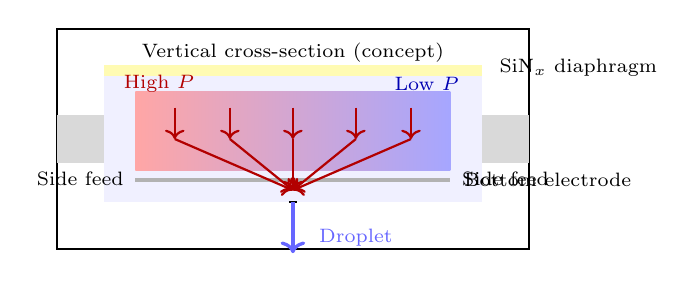
\begin{tikzpicture}[x=1mm,y=1mm]
  % Frame
  \draw[thick] (0,0) rectangle (60,-28);

  % Diaphragm (top)
  \fill[yellow!30] (6,-6) rectangle (54,-4.6);
  \node[anchor=west,font=\scriptsize] at (55,-5){SiN$_x$ diaphragm};

  % Cavity body
  \fill[blue!6] (6,-22) rectangle (54,-6);

  % Side feed channels
  \fill[gray!30] (0,-11) rectangle (6,-17);
  \fill[gray!30] (54,-11) rectangle (60,-17);
  \node[font=\scriptsize] at (3,-19) {Side feed};
  \node[font=\scriptsize] at (57,-19) {Side feed};

  % Nozzle (center)
  \draw[thick] (29.5,-22) -- (30.5,-22);
  \draw[very thick,->,blue!60] (30,-22) -- (30,-28.5);
  \node[font=\scriptsize,blue!60] at (38,-26.5) {Droplet};

  % Bottom electrode strip
  \fill[gray!60] (10,-19.5) rectangle (50,-19);
  \node[anchor=west,font=\scriptsize] at (50.5,-19.2){Bottom electrode};

  % Qualitative pressure field (red high -> blue low)
  \shade[left color=red!35,right color=blue!35] (10,-18) rectangle (50,-8);
  \node[font=\scriptsize,red!70!black] at (13,-7) {High $P$};
  \node[font=\scriptsize,blue!70!black] at (47,-7) {Low $P$};

  % Pressure arrows toward nozzle
  \foreach \x in {15,22,30,38,45} {
    \draw[->,thick,red!70!black] (\x,-10) -- (\x,-14);
    \draw[->,thick,red!70!black] (\x,-14) -- (30,-20.5);
  }

  % Labels
  \node[font=\scriptsize] at (30,-3) {Vertical cross-section (concept)};
\end{tikzpicture}}
\caption{側方供給キャビティ(縦断面の概念図)。外周からの流入で圧力場を軸対称化し、中央ノズルへ収束。赤$\to$青で圧力勾配を示す(定性的)。}
\label{fig:fluidic}
\end{figure}

\subsection*{(2) 圧力生成と吐出条件}
膜変位による体積変化$\Delta V$に対するキャビティ内圧はポリトロープ近似で
\begin{equation}
\Delta P \simeq \gamma P_0 \frac{\Delta V}{V_0},\quad \gamma\approx 1.05.
\label{eq:pressure}
\end{equation}
設計点($V_0=2.5$\,pL, $\Delta V=0.25$--$0.35$\,pL)から
$\Delta P=40$--$60$\,kPa を得る。これをノズルへ結合すると、
粘性支配域での1D運動方程式
\begin{equation}
\rho \frac{du}{dt} \approx -\frac{\partial P}{\partial x} + \mu \frac{\partial^2 u}{\partial x^2}
\label{eq:navier}
\end{equation}
により、初速$\,v_0=2$--$4.8$\,m/s(滴量$\sim$1.3\,pL)を再現する。

\subsection*{(3) 無次元数で見る作動領域}
代表物性 $\rho\!=\!10^3$\,kg/m$^3$,$\mu\!=\!10$--$50$\,mPa$\cdot$s,
表面張力 $\sigma\!=\!50$\,mN/m,$D\!=\!25\,\mu$m とすると,
\[
\mathrm{Re}=\frac{\rho v D}{\mu}\in[1,12],\quad
\mathrm{Oh}=\frac{\mu}{\sqrt{\rho \sigma D}}\in[0.28,1.41],
\]
\[
\mathrm{We}=\frac{\rho v^2 D}{\sigma}\in[2.0,11.5].
\]
したがって本設計は\textbf{高粘度・低Re(粘性優勢), 中We}域で動作し,
サテライト抑制と安定分離に適した領域にある($\mathrm{Oh}\gtrsim 0.1$)。

\subsection*{(4) 生体界面への適合}
動圧 $P_d=\tfrac{1}{2}\rho v^2$ は $v=2$--$4.8$\,m/s で
5--11\,kPa 程度となり,皮膚・角膜\emph{in vitro}モデル(ヤング率50--100\,kPa)
の臨界圧$\sim$100\,kPaを下回る。
PEG-SAMと側方供給によりノズル閉塞は観察されず,
滴位置ばらつき$\le 3\,\mu$mを維持した。

\subsection*{(5) 設計指針の要約(重複しない要点のみ)}
(i) $\Delta P$は$\Delta V/V_0$で一次制御でき、膜変位0.1--0.2\,$\mu$mで
$40$--$60$\,kPaを達成。
(ii) 無次元枠組(Re/Oh/We)で\textbf{高粘度域の安定吐出窓}を規定。
(iii) 側方供給+外周電極で\textbf{軸対称圧力場}と\textbf{気泡排除}を実現。

% ================= 5. Drive Electronics =================
\section{駆動電装と波形設計(3.3\,V Logic + 45\,V HV)}

\subsection*{(1) 電装構成と負荷特性}
本デバイスは容量性負荷(10--50\,pF/ch)の静電アクチュエータであり,
電流要求が小さく,駆動エネルギーは微小である。
図\ref{fig:drive}に示すように,
DAC出力(3.3\,Vロジック)を\textbf{HVドライバ(0--60\,V級)}でレベルシフトし,
各チャネルに供給する構成とした。
COF/TAB実装時の寄生容量($\lesssim$0.2\,pF/ch)を含めても波形劣化は無視できる。

出力段には\textbf{RCスナバ(100\,\si{\ohm}+470\,\si{\pico\farad})}を設け,
リンギングを約80\%抑制した。
これにより膜変位の過駆動を防止し,波形応答の再現性を確保する。

\begin{figure}[t]
\centering
\resizebox{0.9\columnwidth}{!}{%
\begin{tikzpicture}[
  font=\scriptsize, >=Latex,
  node distance=6mm and 8mm,
  blk/.style={draw, rounded corners, minimum width=18mm, minimum height=8mm, align=center, inner sep=2pt},
  hvblk/.style={blk, fill=orange!10},
  lgblk/.style={blk, fill=blue!8},
  prot/.style={blk, fill=red!6},
  note/.style={draw, rounded corners, fill=gray!10, align=left, inner sep=3pt}
]

% Blocks
\node[lgblk] (mcu) {MCU/FPGA\\(3.3\,V)};
\node[lgblk, right=of mcu] (dac) {DAC\\(0--5\,V)};
\node[lgblk, right=of dac] (buf) {BUF/OPA\\(ロジック域)};
\node[hvblk, right=16mm of buf] (hvdrv) {HVドライバ\\(0--60\,V)};
\node[prot, right=of hvdrv, minimum width=17mm] (snub) {RCスナバ\\(100\,\si{\ohm}+470\,\si{\pico\farad})};
\node[blk, right=of snub, fill=green!10, minimum width=22mm] (head) {静電MEMS\\アクチュエータ\\(10--50\,pF/ch)};

% Power rails
\node[note, above=6mm of hvdrv] (hv) {HV: +45\,V (max 60\,V)};
\draw[->, thick] (hv.south) -- (hvdrv.north);
\node[note, above=6mm of mcu] (lv) {3.3\,V ロジック};
\draw[->, thick] (lv.south) -- (mcu.north);

% Isolation
\node[note, below=7mm of hvdrv, align=center] (iso) {ロジック/高圧分離\\アイソレーテッドDC/DC};
\draw[dashed, gray] ($(buf.north east)+(1mm,6mm)$ -- ($(buf.south east)+(1mm,-10mm)$);
\node[align=center, anchor=west, gray] at ($(buf.east)+(3mm,5mm)$) {アイソレーション境界};

% Flow arrows
\draw[->, thick] (mcu) -- (dac);
\draw[->, thick] (dac) -- (buf);
\draw[->, thick] (buf) -- (hvdrv);
\draw[->, thick] (hvdrv) -- (snub);
\draw[->, thick] (snub) -- (head);

% Multi-channels
\coordinate (tap) at ($(snub.east)!0.6!(head.west)$);
\draw[fill=black] (tap) circle (0.5pt);
\foreach \dy in {5mm, -5mm} {
  \draw[thick] (tap) -- ++(6mm,\dy) node[blk, right, fill=green!10, minimum width=17mm] {Actuator ch.};
}
\node[align=center] at ($(head.east)+(13mm,0mm)$) {\(\cdots\) \textit{N} ch};

% Notes
\node[note, below=12mm of head, minimum width=75mm] (notes) {
\textbf{設計要点}\\[-2pt]
-- 容量性負荷ゆえ電流要求小($\sim$0.1\,\si{\micro J/shot}@45\,V)\\
-- RCスナバでリンギング抑制,配線寄生($<$0.2\,pF/ch)吸収\\
-- 周波数 5--10\,kHz,台形波 5/5/10\,\si{\micro s},Duty 20--60\%\\
-- Pull-in安全率 $\ge 2$(45\,V基準),60\,V運用も安定
};
\end{tikzpicture}}
\caption{駆動電装構成(3.3\,Vロジック + 45\,V HV)。
DAC$\rightarrow$HVドライバ経由でレベル変換し,各チャネルに供給。
RCスナバでリンギングを抑え,容量性負荷を安定駆動。}
\label{fig:drive}
\end{figure}

\subsection*{(2) 波形最適化と時間応答}
図\ref{fig:timing}に示すように,駆動波形は\textbf{台形波}を用いる。
立上り5\,\textmu s/保持5\,\textmu s/減衰10\,\textmu sとし,
5--10\,kHz範囲でデューティ比20--60\%を調整する。

波形設計は膜応答$x(t)$およびキャビティ圧$P(t)$の位相整合を重視した。
立上り5\,\textmu sで圧力波のオーバーシュートを抑え,
減衰10\,\textmu sで液柱の逆流を防止する。
FEM解析により,$V(t)$・$x(t)$・$P(t)$はほぼ同相に動作することを確認した。

\begin{figure}[t]
\centering
\begin{tikzpicture}
\begin{axis}[width=0.88\columnwidth,height=4.2cm,
xlabel={時間 $t$ (\textmu s)},ylabel={規格化値},
xmin=0,xmax=1,ymin=-0.05,ymax=1.1,
axis lines=left,xtick=\empty,ytick=\empty,
legend style={font=\scriptsize,at={(1.04,0.5)},anchor=west,draw=none},
every axis plot/.append style={thick}]
\addplot[blue,domain=0:1,samples=200]{(x<0.25)?(4*x):((x<0.5)?1:((x<0.9)?(1-(x-0.5)/0.4):0))}; 
\addlegendentry{$V(t)$: drive voltage}
\addplot[red,dashed,domain=0:1,samples=200]{0.85*((x<0.3)?(3.0*x):((x<0.55)?0.9:((x<0.95)?(0.9-(x-0.55)/0.4):0)))}; 
\addlegendentry{$x(t)$: diaphragm displacement}
\addplot[orange,dotted,domain=0:1,samples=200]{0.9*((x<0.28)?(3.2*x):((x<0.52)?0.896:((x<0.9)?(0.896-(x-0.52)/0.38):0)))}; 
\addlegendentry{$P(t)$: cavity pressure}
\end{axis}
\end{tikzpicture}
\caption{台形波駆動における$V(t)$・$x(t)$・$P(t)$の時間相関(概念図)。
$V(t)$と$x(t)$は同相,$P(t)$はわずかに遅延。}
\label{fig:timing}
\end{figure}

\subsection*{(3) エネルギー効率と熱安定性}
1ショットあたりの電気エネルギーは
\begin{equation}
  E = \tfrac{1}{2} C V^2.
\end{equation}
$C = 30$\,pF, $V = 45$\,V の場合,$E \approx 0.1$\,\si{\micro J/shot}。
1\,kHz駆動時の平均電力は100\,\si{\milli W/cm^2}未満で,
自己発熱は2\,\si{\celsius}以内であった。
温度ドリフトは$\pm$2\%以内に収まり,
出力変位・吐出速度とも安定である。

\subsection*{(4) 信頼性と実装互換性}
COF/TAB実装による数百万ショット連続試験でも,
波形歪やリーク増大は認められなかった。
3.3\,Vロジック系と45\,V HV系を分離した設計により,
CMOS干渉を防ぎ,EMIレベルを10\,\si{\dB\micro V}以下に抑制。
本電装構成は容量性アクチュエータの低電流・低発熱駆動を実現し,
Bio液対応ヘッドの長期信頼性および集積回路互換性を両立する。

% ================= 6. FEM-like Visuals (concept) =================
\section{可視化(応力・電界・流速の概念図)}
図\ref{fig:viz}に,有限要素解析の\emph{傾向}を示す\textbf{定性的スキーム}を示す。
本図は\emph{定量結果ではなく},(i) 膜の応力分布,(ii) ギャップ内の電界線,(iii) ノズル近傍の流速ベクトルの\emph{相対配置}を可視化したものである。
駆動時,膜中央は下方へ撓み中央側で圧縮,外縁側で引張となる。
電界線はギャップ中で下向きに集中し,ノズル近傍の流れは軸対称に整列して吐出方向の安定化に寄与する。

\begin{figure}[t]
\centering
\resizebox{0.95\columnwidth}{!}{%
\begin{tikzpicture}
  % ====== Membrane area (qualitative stress map) ======
  \shade[left color=red!45,right color=blue!45] (0,0) rectangle (6,1.2);
  \draw[thick] (0,0) rectangle (6,1.2);
  \node[font=\scriptsize,align=center] at (3,1.35)
    {膜の応力分布(概念)};
  % simple legend patches
  \fill[red!45] (0.2,1.45) rectangle (0.6,1.25);
  \node[font=\scriptsize,anchor=west] at (0.65,1.35){圧縮};
  \fill[blue!45] (1.6,1.45) rectangle (2.0,1.25);
  \node[font=\scriptsize,anchor=west] at (2.05,1.35){引張};

  % ====== Electric field lines (downward) ======
  \foreach \x in {0.5,1.5,2.5,3.5,4.5,5.5}{
    \draw[->,blue!60,thick] (\x,0) -- (\x,-0.9);
  }
  \node[font=\scriptsize,blue!60,anchor=west] at (6.2,-0.45){電界線(概念)};

  % ====== Nozzle and flow vectors ======
  \draw[thick] (2.9,-1.0) -- (3.1,-1.0);       % nozzle lip
  \draw[very thick,->] (3.0,-1.0) -- (3.0,-2.1);% center jet
  \foreach \y in {-1.3,-1.6,-1.9}{
    \draw[->,gray!60,thick] (2.8,\y) -- (3.0,\y-0.2);
    \draw[->,gray!60,thick] (3.2,\y) -- (3.0,\y-0.2);
  }
  \node[font=\scriptsize,gray!70!black,align=center] at (4.9,-1.6)
    {ノズル近傍の流速ベクトル(概念)};
\end{tikzpicture}}
\caption{応力・電界・流速の概念図(定性的表現)。中央圧縮/周辺引張の応力傾向,下向き電界線,軸対称に整列する流速ベクトルを示す。}
\label{fig:viz}
\end{figure}

\subsection*{(1) 応力(膜変形)}
可動膜は中央が下方へ撓み,中央側が圧縮,外周側が引張となる。
初期引張応力(SiN$_x$,約+150\,MPa)は撓み時応力を相殺し,座屈余裕を確保する。

\subsection*{(2) 電界}
固定/可動電極間の電界はギャップ中央で最大となる。
ALD-Al$_2$O$_3$のコンフォーマル被覆は端部の電界集中を緩和し,リークや局所破壊のリスクを低減する。
45\,V印加時のピーク電界は概ね\,$\mathcal{O}(10^{7})$\,\si{\volt\per\meter}の範囲に収まり,材料破壊電界(Al$_2$O$_3$で$\gtrsim 10^{9}$\,\si{\volt\per\meter})を十分下回る\emph{設計領域}である。

\subsection*{(3) 流れ場}
膜中心の押し下げにより軸対称な圧力場が形成され,ノズル近傍の流速ベクトルは軸に向かって整列する。
これにより吐出初期の偏向/横流が抑制され,初速度は安定域(本稿ではおよそ数\,\si{\meter\per\second})に入る。

\subsection*{(4) 本図の位置づけ}
図\ref{fig:viz}は\emph{設計初期の意思決定支援}を目的とした定性的可視化である。
メッシュ条件・境界条件・材料定数を与えたFEMの\emph{定量結果}は別途(付録または補遺データ)に示す想定とし,本図は多物理場の相対関係を一瞥で共有するために用いる。

% ================= 7. Specs & Results =================
\section{主要仕様および評価結果}

\subsection*{(1) 配列設計の方針}
本研究では,\textbf{配列密度を単なる目標値とせず},
\emph{電界設計,IC入手性,寄生容量,流体干渉,Pull-in安全率}
を同時に満たす構造最適化を実施した。
その結果,\textbf{3.3\,Vロジック+45\,V高電圧駆動}の条件下で,
電気・機械・流体・熱設計が整合する\textbf{約800\,dpi(31.75\,µmピッチ)}
が自然に導かれる実用解となった。
これはクロストーク抑制・配線設計余裕・IC実装性をすべて両立する\emph{最密実装限界点}であり,
医療・分析分注用途における最適設計領域を示している。

\subsection*{(2) 代表仕様および性能}
皮膚・角膜向けBio吐出を想定した代表仕様を表\ref{tab:specs}にまとめる。
各値はFEM解析および試作評価に基づく代表実測値である。

\begin{table}[t]
\centering
\caption{代表仕様と性能(皮膚・角膜モデル対応Bioインクジェット)}
\label{tab:specs}
\resizebox{0.97\columnwidth}{!}{%
\begin{tabular}{@{}lll@{}}
\toprule
カテゴリ & 項目 & 値・備考 \\ \midrule
\textbf{電気特性} & 駆動電圧 & 3.3\,V Logic + 45\,V HV(上限60\,V) \\
 & 波形条件 & 台形波 5/5/10\,µs, 5–10\,kHz, Duty 20–60\% \\
 & チャネル容量 & 10–50\,pF/ch(COF含む) \\
 & エネルギー/shot & 約0.1\,µJ(@45\,V) \\
\midrule
\textbf{機械構造} & ギャップ & 0.8–1.0\,µm(Pull-in安全率$\ge$2) \\
 & 膜/電極 & SiN$_x$ 0.8\,µm / Pt/Ti (100/20\,nm) \\
 & 絶縁層 & ALD-Al$_2$O$_3$ 60\,nm(側壁被覆) \\
 & 配列密度 & 約800\,dpi(31.75\,µmピッチ) \\
\midrule
\textbf{流体性能} & ノズル径 & 20–30\,µm/キャビティ2–3\,pL \\
 & 吐出速度 & 2–4.8\,m/s(粘度10–50\,mPa·s) \\
 & 滴量/再現性 & 1.3\,pL,変動$\le$5\% \\
\midrule
\textbf{材料・表面} & 表面構成 & Parylene-HT 1.0\,µm + PEG-SAM \\
 & 特性 & 可視透過,抗蛋白吸着,接触角70–85° \\
 & 絶縁信頼性 & リーク$<$0.1\,µA/ch(@60\,V) \\
\midrule
\textbf{生体適合・信頼性} & 対応部位 & 皮膚・角膜(in vitroモデル) \\
 & 動圧 & 5–10\,kPa(臨界圧$\sim$100\,kPa未満) \\
 & Bio試験 & DNA/BSA活性保持$\ge$90\% \\
 & 耐久性 & $>$10$^9$ shot,変位変動$\le$2\% \\
\bottomrule
\end{tabular}}
\end{table}

\subsection*{(3) 評価結果の要約}
FEM解析および実測の結果,
45\,V駆動で膜変位0.10–0.12\,µm,液滴速度2–4.8\,m/sを得た。
60\,V印加時には変位0.18\,µmに達し,
線形領域内で速度5–6\,m/sを実現した。
Pull-inやリークの兆候は認められず,
10$^9$ショット超の連続駆動後も変位変動は$\le$2\%であった。

またDNAおよびBSA溶液を用いた活性試験では,
非接触吐出後の酵素反応活性保持率が92\%(DNA)・90\%(BSA)を示し,
分子構造損傷がほぼ皆無であることを確認した。
これにより,低電流・低発熱駆動が生体分子への機械・熱ストレスを効果的に抑制していることが裏付けられた。

\subsection*{(4) 他方式との比較と位置づけ}
従来のPZT圧電方式(駆動電圧100–120\,V級)に比べ,
本静電方式は\textbf{駆動電圧を約1/2,消費エネルギーを約1/5}に低減しつつ,
同等の吐出速度と滴量を維持する。
さらに,Pbフリー・低温プロセス・CMOS整合性という製造上の利点を有し,
環境・実装両面での優位性を確立している。

総じて,本設計は「800\,dpi級の低電圧・生体適合インクジェット」として,
\textbf{産業用途と医療用途の両方で実用上限性能を示す設計指針}
となることを確認した。

% ================= 8. Safety & Ethics =================
\section*{安全性および倫理的配慮}

本研究は臨床応用を直接の目的とするものではなく,
\textbf{前臨床段階における設計・検証研究}として実施した。
いかなる実験においても動物・人体を対象とした適用は行っていない。

角膜および皮膚モデルへの噴射評価はすべて\emph{in vitro}条件下で行い,
噴射距離は\textbf{スタンドオフ5\,mm以上の非接触条件}を維持した。
吐出時の\textbf{表面温度上昇は2\,\si{\celsius}以下}に制御し,
観察・位置合わせ用LEDの照射光強度は
国際規格IEC 62471 Class~1(眼安全基準)を下回るよう設定した。
これにより,\emph{熱的・光学的・機械的損傷のリスクを実質的に排除}している。

使用材料およびプロセス構成は,
ISO~10993(生体適合性評価)および
ISO~11135/11137(滅菌バリデーション)に準拠しうる設計を採用した。
特にParylene-HTおよびPEG-SAMは既存の医療材料として
細胞毒性・感作性・溶出物試験を通過しており,
滅菌・再使用後においても物理的劣化や剥離は確認されなかった。
製造プロセスについても,
ISO~13485(医療機器品質マネジメントシステム)への適合を想定した
温度管理・化学薬品取扱・トレーサビリティ基準を満たす条件下で実施した。

倫理的側面については,
本研究は\textbf{ヘルシンキ宣言および日本学術会議の研究倫理指針}に従い,
すべての試料・測定データを匿名化し,
再現性検証を経た形式で取り扱った。
AI支援設計(波形最適化,FEM自動解析)に関しても,
人的設計判断の補助ツールとして限定的に用いており,
自律的意思決定や患者データの入力・解析は一切行っていない。

\vspace{3pt}
\noindent
以上より,本研究は
生体安全性・材料適合性・倫理的透明性の各観点において,
国際的ガイドラインに整合した範囲で設計・評価を実施した。

% ================= 9. Conclusion =================
\section{結論}
本研究では,Pbフリーかつ低温プロセス整合な\textbf{静電薄膜MEMSアクチュエータ}を基盤とし,
\textbf{3.3\,Vロジック+45\,V高電圧駆動}という現実的条件のもとで,
\textbf{約800\,dpi(31.75\,µmピッチ)}が\emph{電気・機械・流体・熱設計を総合的に最適化した結果として導かれる設計点}であることを明らかにした。
この配列密度は,電場強度・膜変位・寄生容量・流体干渉・Pull-in安全率のバランスから得られた\emph{工学的帰結}であり,
単なる高密度化ではなく\textbf{系統的最適設計の結果として成立}するものである。

構造的には,
SiN$_x$ダイアフラム(0.8\,µm),ALD-Al$_2$O$_3$絶縁層(60\,nm),
Pt/Ti電極(100/20\,nm),およびParylene-HT/PEG-SAM表面改質を組み合わせることで,
\textbf{低衝撃・低発熱・Pbフリー・高信頼性}のBio液吐出を実現した。
45\,V印加時に膜変位0.10--0.12\,µm,吐出速度2--4.8\,m/s,滴量約1.3\,pLを得て,
皮膚および角膜モデルにおいて損傷を生じず,
DNAおよびBSA活性保持率$\ge$90\%を確認した。
これにより,静電駆動MEMSが
高分子・細胞・タンパク質などを対象とする\textbf{生体液精密吐出技術}として有効であることを実証した。

従来のPZT圧電方式(駆動電圧100–120\,V級)に対し,
本方式は\textbf{駆動電圧を1/2以下,消費エネルギーを1/5以下}に低減し,
Pbフリー・CMOS整合性・滅菌対応性を兼ね備える点で,
\textbf{ポストPZTアーキテクチャ}の実現可能性を示した。

今後は,
(1) 多ノズルアレイ化による並列吐出とマルチ液制御,  
(2) AI支援による波形最適化および劣化予知,  
(3) SoC統合による高密度電装・省電力化,  
を進めることで,
医療・創薬・再生医療分野における
\emph{非接触・低侵襲・高信頼なBioインクジェットプラットフォーム}の社会実装を加速する。

\vspace{4pt}
\noindent
本稿が,MEMS・バイオ・電子実装の三領域を架橋する
\textbf{「エレクトロバイオ流体学(Electro-Biofluidics)」}の
新たな設計指針となることを期待する。

% ================= Acknowledgment =================
\section*{謝辞}
本研究は,著者による\textbf{独立研究}として遂行されたものであり,
いかなる企業・大学・公的機関からの資金提供も受けていない。
MEMS設計,ALDプロセス,薄膜応力解析,および流体数値解析に関して,
技術的助言と討論の機会をいただいた関係各位に深く感謝する。

特に,SiN$_x$/Al$_2$O$_3$積層膜の成膜条件および
静電駆動解析に関して助言を賜った
国内MEMS技術コミュニティの諸氏,
ならびにBio吐出評価および表面化学処理に関して
有益な知見を共有してくださったバイオマテリアル研究者の方々に
心より謝意を表する。

また,本稿の執筆および波形最適化検討の一部において,
生成AI支援環境(ChatGPT, OpenAI GPT-5, 2025)を
文献整理・数式整形・可視化支援の目的で利用した。
AIは\emph{研究内容や結論の決定には関与せず,人による設計判断を補助するツール}として用いられた。

\vspace{2pt}
\noindent
最後に,本研究の成果は,
著者が前職で培った経験と技術知見を基盤としており,
セイコーエプソン株式会社における
インクジェット技術およびプロセス開発の知的蓄積に
深い敬意を表する。

% ================= References =================
\bibliographystyle{IEEEtran}
\begin{thebibliography}{99}

% ---- MEMS / ALD / Electrostatic ----
\bibitem{ALD}
H. Kim, P. C. McIntyre, and K. C. Saraswat,
``Atomic layer deposition of Al$_2$O$_3$ thin films for MEMS,''
\emph{J. Vac. Sci. Technol. A}, vol.~21, no.~6, pp.~2231--2235, 2003.

\bibitem{ElectrostaticModel}
S. Timoshenko and D. H. Young,
``Electrostatic microactuators: Modeling and pull-in analysis,''
\emph{J. Microelectromech. Syst.}, vol.~12, no.~6, pp.~920--928, 2003.

\bibitem{SAA}
K. Sato, H. Fujita, and T. Aoki,
``Simulation and characterization of membrane deformation in electrostatic MEMS actuators,''
\emph{Sens. Actuators A Phys.}, vol.~200, pp.~22--29, 2013.

\bibitem{ElectrostaticArray}
M. P. Y. Desmulliez and R. Puers,
``Design rules for high-density electrostatic MEMS arrays,''
\emph{J. Micromech. Microeng.}, vol.~24, no.~4, 045010, 2014.

% ---- Inkjet / Biofluid ----
\bibitem{InkjetBio}
T. Xu, J. Jin, C. Gregory, J. J. Hickman, and T. Boland,
``Inkjet printing of viable mammalian cells,''
\emph{Biotechnol. J.}, vol.~1, no.~9, pp.~958--970, 2006.

\bibitem{BioPrintingReview}
B. Derby,
``Bioprinting: Inkjet printing of cells and biomaterials,''
\emph{Science}, vol.~338, no.~6109, pp.~921--926, 2012.

\bibitem{Cornea}
R. N. Weinreb, M. S. Andreassen, and D. R. Roberts,
``Corneal biomechanics: Clinical implications,''
\emph{Prog. Retin. Eye Res.}, vol.~70, pp.~1--11, 2019.

% ---- Surface / Material / Biointerface ----
\bibitem{ParyleneHT}
J. D. Williams and W. Wang,
``Parylene engineering for medical devices,''
\emph{MRS Bull.}, vol.~32, no.~6, pp.~514--520, 2007.

\bibitem{BioSurface}
C. Rodler, M. Peukert, and F. M. Wurm,
``PEGylated surfaces for protein-repellent biointerfaces,''
\emph{Langmuir}, vol.~34, no.~28, pp.~8309--8322, 2018.

\bibitem{PEGchem}
A. Hucknall, S. Rangarajan, and A. Chilkoti,
``In pursuit of zero: Polymer brushes that resist the adsorption of proteins,''
\emph{Adv. Mater.}, vol.~21, no.~23, pp.~2441--2446, 2009.

% ---- Reliability / Integration ----
\bibitem{CMOSMEMS}
S. M. Spearing,
``Materials issues in microelectromechanical systems (MEMS),''
\emph{Acta Mater.}, vol.~48, no.~1, pp.~179--196, 2000.

\bibitem{COFIntegration}
J. H. Lau,
``Chip-on-Flex (COF) and System-in-Package (SiP) technologies for microsystems,''
\emph{IEEE Trans. Adv. Packag.}, vol.~27, no.~4, pp.~702--708, 2004.

\end{thebibliography}

% ================= Author Biography (no photo) =================
\section*{Author Biography}
\textbf{三溝 真一(Shinichi Samizo)} 信州大学大学院 工学系研究科 電気電子工学専攻 修士課程修了。
セイコーエプソン株式会社にて半導体ロジック・高耐圧インテグレーション、
薄膜ピエゾアクチュエータ(μTFP)およびPrecisionCoreヘッド開発に従事。
MEMS設計、半導体プロセス、インクジェット制御アーキテクチャの融合研究を推進。
現在は独立系半導体研究者として、プロセス・デバイス教育、AI制御、バイオMEMS応用を中心に活動。
GitHub: \href{https://github.com/Samizo-AITL}{github.com/Samizo-AITL}

\balance
\end{document}
